\documentclass[
	paper=a4,				% Papierformat
	twoside=true,			% Zweiseitiges Layout
	BCOR=6mm,				% Rand zum Binden
	fontsize=12pt,			% Schriftgröße
	pagesize=auto,			% Schreibt die Papiergröße korrekt ins Ausgabedokument
	numbers=noenddot,		% Kein Punkt nach der Kapitel-Nummer
	bibliography=totoc,		% Quellenverzeichnis im Inhaltsverzeichnis auflisten
	draft=false
]{scrartcl}
% siehe http://tex.stackexchange.com/questions/183149/cant-silence-a-pdftex-pdf-inclusion-multiple-pdfs-with-page-group-error
\pdfsuppresswarningpagegroup=1
% Legt die Zeichenkodierung fest, z.B UTF8
\usepackage[utf8]{inputenc}
% Erweiterten Zeichensatz für europäische Sprachen aktivieren
\usepackage[T1]{fontenc}
% Silbentrennung nach neuer deutscher Rechtschreibung
\usepackage[ngerman]{babel}
% Beseitigt Probleme mit noch nicht vollständig aktualisierten Paketen (z.B. listings)
\usepackage{scrhack}
% Zum flexiblen Einbinden von Grafiken, pdftex ist optional
\usepackage[pdftex]{graphicx}
% Umgebung um mehrere Abbildungen zu einer zu kombinieren
\usepackage{subfig}
% Führt die SCfigure-Umgebung ein (Caption neben der Abbildung)
\usepackage{sidecap}
\renewcommand{\sidecaptionrelwidth}{2.0}
% Damit kann ein Bild vom Text umflossen werden
\usepackage{wrapfig}
% Darstellung für Caption s.u.
\usepackage[font=small,labelfont=bf,labelsep=colon,format=plain]{caption}
\usepackage{amsmath}
\usepackage{amssymb}
\usepackage{cite}
% Verbessert die Kompatibilität von siunitx mit microtype
\usepackage{textcomp}
\usepackage{siunitx}
\sisetup{
	output-decimal-marker = {,},
	per-mode = symbol,
	list-final-separator = { und },
	list-pair-separator = { und },
	range-phrase = { bis },
}
\usepackage{listings}
% Umlaute in Listings sind nur mit folgender Option möglich:
\lstset{
    literate={ö}{{\"o}}1
    {ä}{{\"a}}1
    {ü}{{\"u}}1
}
% Standard-Werte für Listings festlegen:
\lstset{
    frame=single,
    flexiblecolumns=true,
    commentstyle=\color{darkgreen},
    float,
    basicstyle=\small\sffamily,
    numbers=left,
    numberstyle=\tiny,
    showstringspaces=false,
    keepspaces,
    tabsize=4
}
% Zum Einfärben von Code:
\usepackage{color}
\definecolor{darkgreen}{rgb}{0,0.5,0}

% Fußnoten formatieren und Unterstützung für aufeinander folgende Fußnoten:
\usepackage[flushmargin,multiple]{footmisc}
% Hurenkinder und Schusterjungen komplett verbieten:
%\clubpenalty = 10000
%\widowpenalty = 10000
%\displaywidowpenalty = 10000
%\usepackage{microtype}
% Hyperlinks erstellen, wobei Fußnoten aus Kompatibilitätsgründen ausgenommen werden:
\usepackage[hyperfootnotes=false,pdfpagelabels]{hyperref}

% subsubsections werden nummeriert (Standard: subsections)
\setcounter{secnumdepth}{\subsubsectionnumdepth}

% Platz für 3 stellige Seitenzahlen im Inhaltsverzeichnis schaffen:
\makeatletter
\renewcommand{\@pnumwidth}{3em} 
\renewcommand{\@tocrmarg}{4em}
\makeatother

% Schriftgröße der Bildunterschriften verkleinern:
\addtokomafont{caption}{\small\linespread{1}\selectfont}
% Zweite Zeile der Bildunterschrift einrücken:
\setcapindent{1em}

\begin{document}	

\author{Michael Entrup}
\title{Anhang B \\ Die Parameter \texttt{SpecMag} und \texttt{QSinK7}}
\date{April 2017}

\maketitle

% Inhaltsverzeichnis
\tableofcontents

\section{Der Parameter \texttt{SpecMag}} \label{append:Characterisierung-SpecMag}

\begin{figure}
	\centering
	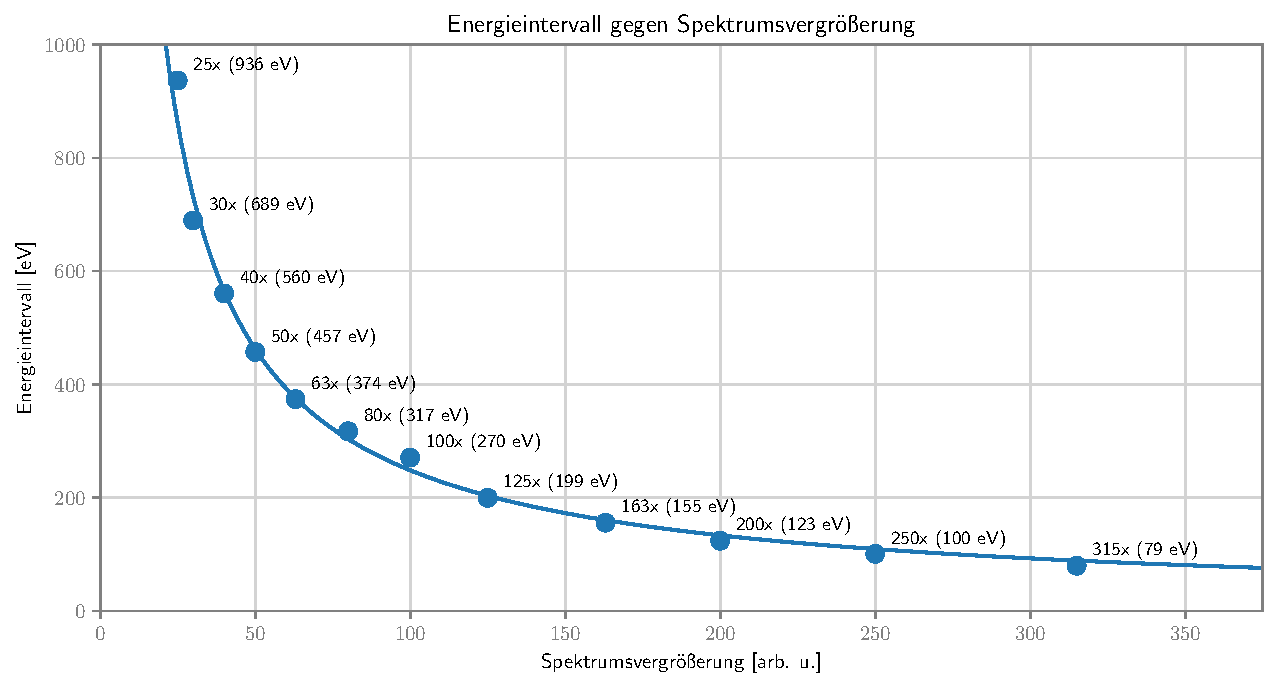
\includegraphics[width=1\linewidth]{../../Jupyter-Notebooks/Kapitel1/Bilder/Intervall_vs_SpecMag}
	% siehe 'EELS-SpecMag.ipynb'
	\caption{Abhängigkeit des abgebildeten Energieintervalls von der eingestellten Spektrumsvergrößerung. Neben den diskreten Werten ist eine Potenzfunktion ($f(x) = a\cdot x^{-r}$) eingezeichnet. Zu erwarten wäre $r=1$ ($\frac{1}{x}$-Abhängigkeit), wovon der ermittelte Wert ($r\approxeq\num{0,9}$) etwas abweicht.}
	\label{fig:SpecMag}
\end{figure}

Dieser Abschnitt soll zeigen, dass \texttt{SpecMag} keinen Einfluss auf die Verzeichnung der SR-EEL Spektren hat. Durch das Skalieren von Aufnahmen bei unterschiedlichen \texttt{SpecMag}-Werten wird die Übereinstimmung der Verzeichnung überprüft.

Wir legen fest, dass ein \texttt{SpecMag}-Wert von \SI{315}{x}\footnote{Dieser Wert wurde gewählt, weil es die höchste Spektrumsvergrößerung ist, welche eingestellt werden kann. Da wir die kleinste einstellbare Vergrößerung nicht nutzen, ist es nicht sinnvoll, diese als Basiskoordinatensystem zu verwenden.} unser Basiskoordinatensystem vorgibt. Die Koordinaten der anderen Messungen werden so skaliert, dass die geringere Vergrößerung dadurch kompensiert wird. Beeinflusst der SpecMag-Wert nur die Vergrößerung, so sollten sich die skalierten Ergebnisse gleichen, wenn die Position der Filtereintrittsblende zwischen den Messungen nicht geändert wurde.

\begin{figure}
	\centering
	\subfloat[keine Skalierung]{%
		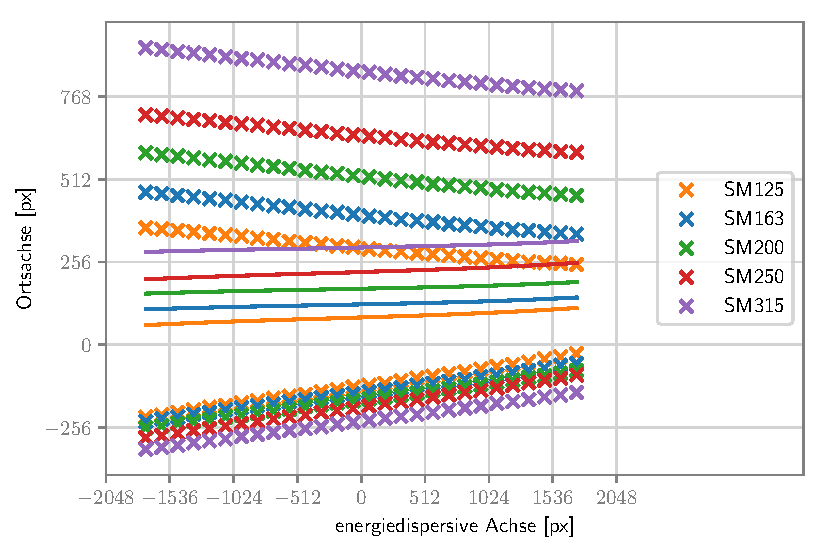
\includegraphics[width=.49\linewidth]{../../Jupyter-Notebooks/AnhangB/Bilder/SR-EELS_Charakterisierung_Vergleich_SM}
		\label{fig:SR-EELS_Charakterisierung_Vergleich_SM_raw}
	}
	\subfloat[Skalierung der Vergrößerung]{%
		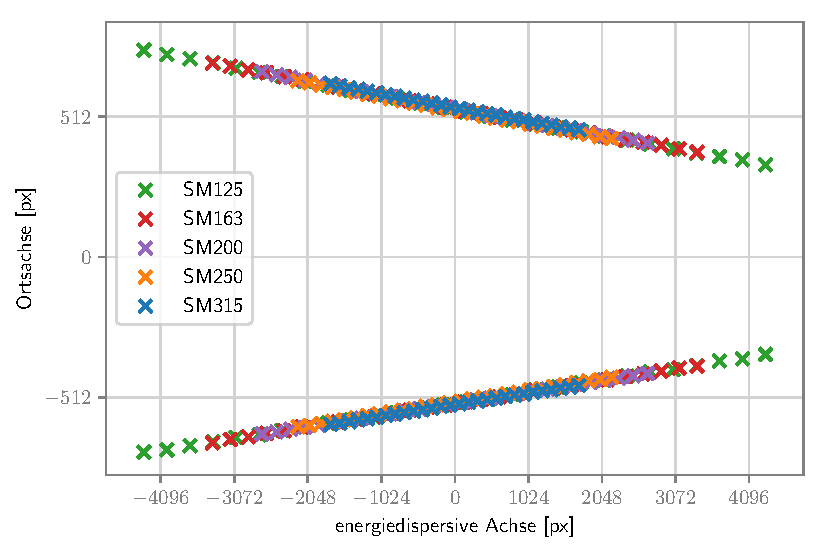
\includegraphics[width=.49\linewidth]{../../Jupyter-Notebooks/AnhangB/Bilder/SR-EELS_Charakterisierung_Vergleich_SM_scaled}
		\label{fig:SR-EELS_Charakterisierung_Vergleich_SM_scaled}
	}
	\caption[SR-EEL Spektren bei unterschiedlichen Vergrößerungen]{SR-EEL Spektren bei unterschiedlichen Vergrößerungen und identischer Blendenposition. \subref{fig:SR-EELS_Charakterisierung_Vergleich_SM_raw} zeigt die Ausdehnung der Spektren, wie sie von der Kamera aufgenommen wurden. Die durchgezogenen Linien stellen jeweils das Zentrum der einzelnen Spektren dar. Bei \subref{fig:SR-EELS_Charakterisierung_Vergleich_SM_scaled} wurden die Spektren entsprechend der verwendeten Vergrößerung skaliert und das Zentrum als 0 auf der y-Achse gewählt.}
	\label{fig:SR-EELS_Charakterisierung_Vergleich_SM}
\end{figure}

Abbildung \ref{fig:SR-EELS_Charakterisierung_Vergleich_SM_raw} zeigt die Ausdehnung der SR-EEL Spektren für 5 verschiedene Vergrößerungen des Spektrums (\texttt{SpecMag} abgekürzt als SM), wobei noch keine Skalierung durchgeführt wurde. Für eine hohe Vergrößerung zeigt sich eine größere Ausdehnung, als für eine geringe Vergrößerung. Es ist außerdem zu erkennen, dass die Spektren auf der y-Achse leicht zueinander verschoben sind. Dies zeigt sich deutlicher an den durchgezogenen Linien, welche jeweils das Zentrum eines Spektrums markieren. Die Koordinaten beziehen sich auf die Pixel der Kamera, wobei das Zentrum der Kamera als Ursprung gewählt wurde.

Durch die Kalibrierung der energiedispersiven Achse sind die Vergrößerungen zwischen den einzelnen \texttt{SpecMag}-Werten bekannt (siehe Abbildung \ref{fig:SpecMag}). Damit lassen sich die in Abbildung \ref{fig:SR-EELS_Charakterisierung_Vergleich_SM_raw} gezeigten Ausdehnungen auf eine einheitliche Vergrößerung skalieren. Um die Verschiebung der Spektren zu kompensieren, wird nur die Position der Ränder, bezogen auf das Zentrum des jeweiligen Spektrums, betrachtet. Dadurch ergeben sich die in Abbildung \ref{fig:SR-EELS_Charakterisierung_Vergleich_SM_scaled} gezeigten Positionen für den oberen Rand und den unteren Rand der Spektren. Es zeigt sich, dass die zu Beginn des Abschnitts geäußerte Vermutung zutrifft. Eine höhere Vergrößerung des Spektrums stellt einen Ausschnitt der energiedispersiven Ebene mit erhöhter Auflösung dar und dabei keinen Einfluss auf die Verzeichnung. Leider tritt eine Verschiebung entlang der Ortsachse auf, was wir Abbildung \ref{fig:SR-EELS_Charakterisierung_Vergleich_SM_raw} entnehmen können.

Die Verschiebung entlang der Ortsachse hängt mit der Realisierung des EELS-Modus am Zeiss Libra 200FE zusammen. Schaltet man in den EELS-Modus, so steht dem Nutzer die Möglichkeit zur Verfügung, den ZLP des Spektrums in das Zentrum der Kamera zu verschieben. Dazu verwendet man die \glqq Spec Shift\grqq\ genannte Funktion, mit der man das Abbild der energiedispersiven Ebene auf der energiedispersiven Achse und auf der Ortsachse verschieben kann. Für jede Vergrößerung (\texttt{SpecMag}) lassen sich Offset-Werte hinterlegen, die dafür sorgen sollen, dass das Spektrum sich beim Wechsel der Vergrößerung (\texttt{SpecMag}) nicht verschiebt. Leider sind die hinterlegten Werte nicht mehr korrekt, wodurch sich die kleine Verschiebung ergibt. Entlang der energiedispersiven Achse können wir mit der verwendeten Methode keine Verschiebung feststellen. Aufnahmen von EEL Spektren zeigen jedoch, dass für die hier betrachteten Vergrößerungen (\texttt{SpecMag}) keine Verschiebung auftritt. Dies ist damit zu erklären, dass die Offset-Werte von \glqq Spec Shift\grqq\ sehr wahrscheinlich bei der Aufnahme von EEL Spektren justiert wurden und dort nur die energiedispersive Achse von Bedeutung ist.

\section{Der Parameter \texttt{QSinK7}} \label{append:Characterisierung-QSinK7}

Die Auswirkungen des Parameters \texttt{QSinK7} auf die Verzeichnung der SR-EEL Spektren wurden im Rahmen dieser Arbeit detailliert untersucht. An zwei Beispielen sollen die Ergebnisse exemplarisch besprochen werden. Im Jupyter-Notebook, das für die Auswertung verwendet wurde, sind zusätzliche Diagramme zu finden.\footnote{\url{https://github.com/m-entrup/Dissertation/blob/master/Jupyter-Notebooks/Kapitel3/SR-EELS-Charakterisierung-QSinK7.ipynb}}
Für diese Auswertung standen mehr als 80 Messreihen zur Verfügung. Die Messreihen verteilen sich auf sechs verschiedene \texttt{SpecMag}-Werte: \SI{100}{x}, \SI{125}{x}, \SI{163}{x}, \SI{200}{x}, \SI{250}{x} und \SI{315}{x}. Jede Messreihe besteht dabei aus 3 bis 19 Einzelmessungen.

Die Abhängigkeit der mittleren Breite eines SR-EEL Spektrums von der mittleren Position auf der Ortsachse ist ein Abbildung \ref{fig:SR-EELS_Charakterisierung_QSinK7_SM315_Pos} gezeigt. Jede Kurve entspricht einem Wert von \texttt{QSinK7}, wobei mehr als eine Messreihe zu einem \texttt{QSinK7}-Wert beitragen kann (bei \SI{-11}{\percent} sind es zwei Messreihen und bei \SI{0}{\percent} sind es drei Messreihen). Jeder Datenpunkt in einem der Diagramme resultiert aus einer Einzelmessung. Zu jedem \texttt{QSinK7}-Wert wurde ein Fit mit einem Polynom zweiten Grades durchgeführt, um die Abhängigkeit der Breite von der Position besser sichtbar zu machen. Für \texttt{QSinK7} = \SI{-8}{\percent} stimmt diese Funktion sehr gut mit der Lage der Datenpunkte überein, da die Datenpunkte von der gleichen Messreihe stammen. Weiterhin fällt auf, dass die Maxima der mittleren Breite an unterschiedlichen Positionen auftreten. Dies hat nichts mit den gewählten Wert von \texttt{QSinK7} zu tun. Da die Messungen zu unterschiedlichen Zeitpunkten durchgeführt wurden, konnte nicht gewährleistet werden, dass der Parameter \glqq Spectrum Shift\grqq\ identisch ist, denn von der Software wird kein numerischer Wert ausgegeben.


\subsection{Abhängigkeit der Breite von QSinK7} \label{append:Characterisierung-Width-vs-QSinK7}

Der aus den verschiedenen Messreihen erstellte Datensatz ermöglicht die Untersuchung diverser Zusammenhänge. Ein interessanter Zusammenhang ergibt sich bei der Betrachtung der mittleren Breite in Abhängigkeit von \texttt{QSinK7}. Die Abbildungen \ref{fig:SR-EELS_Charakterisierung_QSinK7_SM125_QSinK7} und \ref{fig:SR-EELS_Charakterisierung_QSinK7_SM315_QSinK7} zeigen einen linearen Zusammenhang für SpecMag \SI{125}{x} und \SI{315}{x}. Im Anhang \ref{append:Characterisierung-QSinK7} sind Diagramme für zwei weitere SpecMag-Werte (\SI{100}{x} und \SI{200}{x}) zu finden und auch dort ist ein linearer Zusammenhang gegeben. Eine Ausgleichsgerade ist nur für negative Werte von \texttt{QSinK7} und \SI{0}{\percent} eingezeichnet, da nur dafür ausreichend Messungen durchgeführt wurden. Abbildung \ref{fig:SR-EELS_Charakterisierung_QSinK7_SM200_QSinK7} zeigt jedoch, dass auch bei positiven Werten von \texttt{QSinK7} ein linearer Zusammenhang gegeben ist.

Auf die Wahl des optimalen \texttt{QSinK7} hat diese Erkenntnis keine Auswirkung, da wir den Wert verwenden möchten, bei dem die Variation der Breite am geringsten ist. Die lineare Abhängigkeit könnte jedoch hilfreich sein, wenn man zu einem bisher nicht charakterisierten Wert von \texttt{QSinK7} die Vergrößerung bestimmen möchte. Kennt man schon die Vergrößerung von zwei anderen \texttt{QSinK7}-Werten, so lässt sich die Vergrößerung des neuen Wertes interpolieren. Außerdem lässt sich auf diese Weise abschätzen, wie stark die Vergrößerung im Vergleich zum Abbildungsmodus reduziert ist. Dort erhalten wir für die \SI{100}{\mu\meter}-Blende, welche auch für die Charakterisierung von SR-EELS verwendet wird, einen Durchmesser von etwa \SI{1050}{Pixel}. In Abbildung \ref{fig:SR-EELS_Charakterisierung_QSinK7_SM125_QSinK7_norm} ist die Vergrößerung von SR-EELS als Relativwert, im Vergleich zum Abbildungsmodus aufgetragen.


\subsection{Auswirkung von QSinK7 auf den Abbildungsmodus}

\begin{figure}
	\centering
	\subfloat[$\mathrm{QSinK7}=\SI{0}{\percent}$]{%
		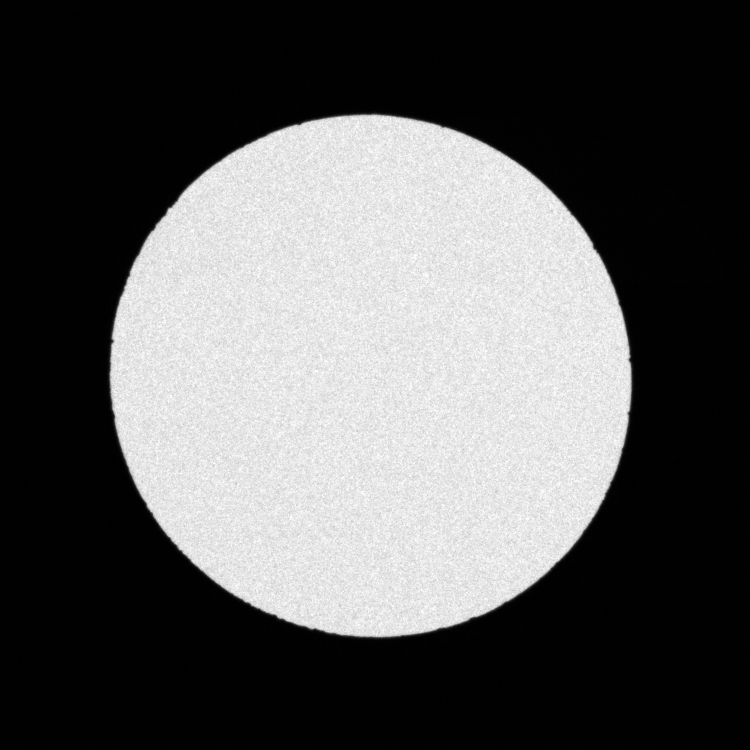
\includegraphics[width=.49\textwidth]{Bilder/SR-EELS_Blende_QSinK7=0}
		\label{fig:SR-EELS_Blende_QSinK7=0}
	}
	\subfloat[$\mathrm{QSinK7}=\SI{-33}{\percent}$]{%
		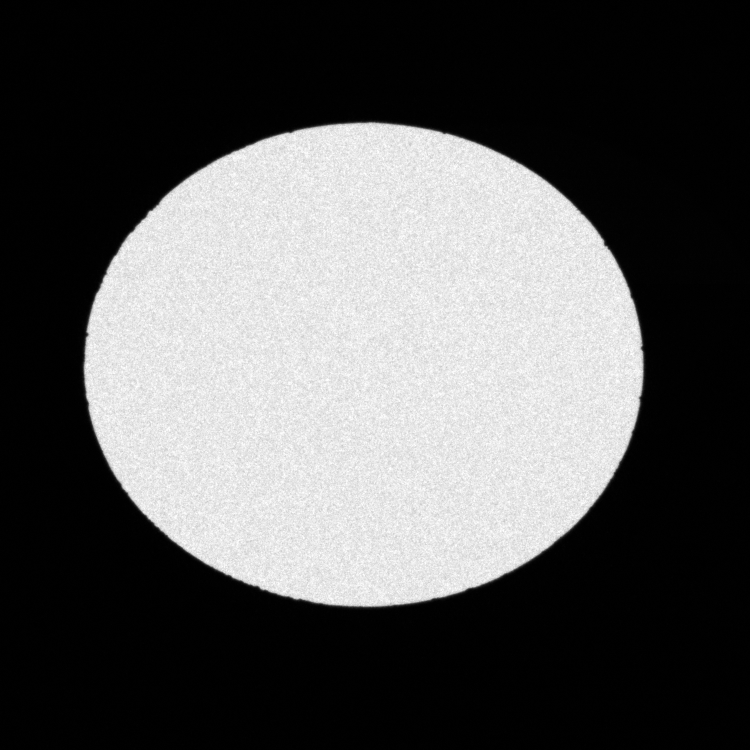
\includegraphics[width=.49\textwidth]{Bilder/SR-EELS_Blende_QSinK7=-33}
		\label{fig:SR-EELS_Blende_QSinK7=-33}
	}
	\caption{Einfluss des Parameters QSinK7 auf den Abbildungsmodus, am Beispiel von Aufnahmen der Filtereintrittsblende.}
	\label{fig:fig:SR-EELS_Blende_QSinK7}
\end{figure}

Ändert man den Parameter QSinK7, so hat dies außerdem Auswirkungen auf den Abbildungsmodus. Die Abbildungen \ref{fig:fig:SR-EELS_Blende_QSinK7} zeigen Aufnahmen der Filtereintrittsblende bei Verwendung von $\mathrm{QSinK7}=\SI{0}{\percent}$ und $\mathrm{QSinK7}=\SI{-33}{\percent}$. Bei $\mathrm{QSinK7}=\SI{0}{\percent}$ beträgt das Verhältnis von größtem Radius zu kleinstem Radius \num{1,02}. Dieses Verhältnis erhöht sich auf \num{1,16}, wenn $\mathrm{QSinK7}=\SI{-33}{\percent}$ verwendet wird. Die Gesamtintensität ist bei beiden Abbildungen identisch (\SI{0,08}{\percent} Unterschied).

Aus dieser Beobachtung lässt sich folgern, dass QSinK7 auf \SI{0}{\percent} zurückgesetzt werden muss, bevor man im Abbildungsmodus arbeitet. Macht man dies nicht, so weisen die Abbildungen eine deutliche Verzerrung auf, die eine quantitative Auswertung der Abstände und Größen von Objekten verfälscht.

\clearpage

\begin{figure}
	\centering
	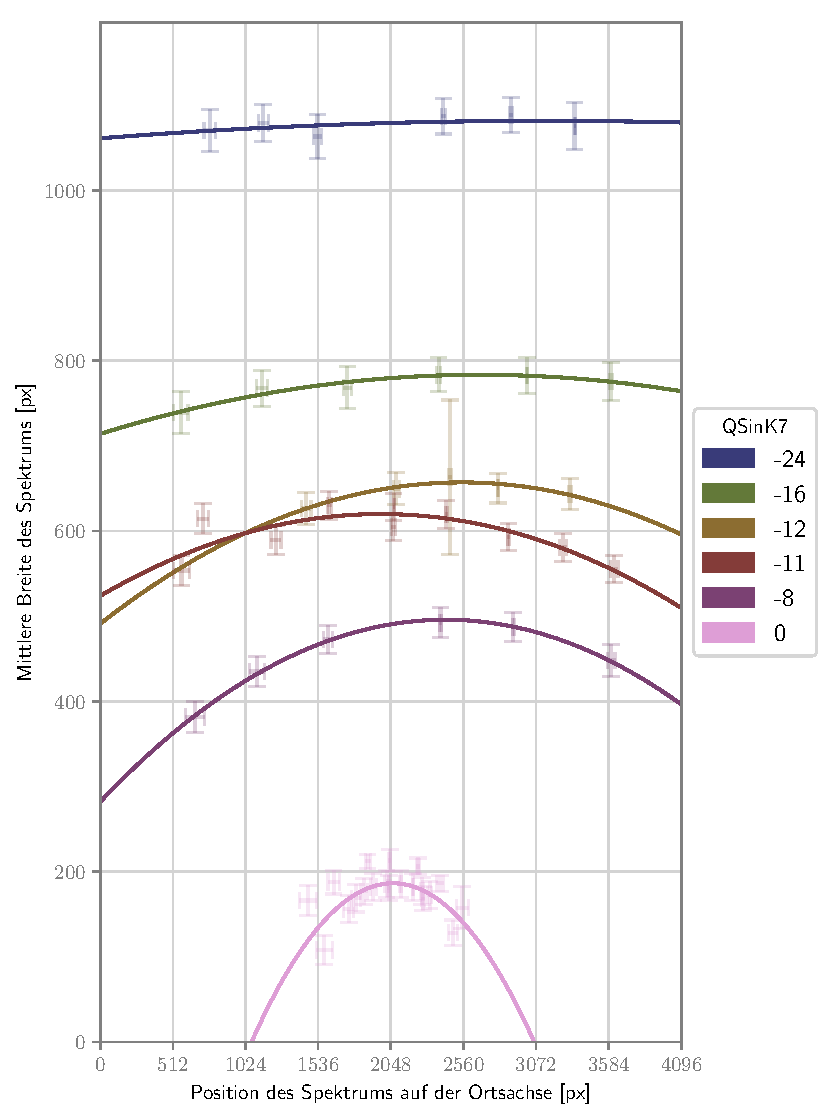
\includegraphics[width=.9\linewidth]{../../Jupyter-Notebooks/Kapitel2/Bilder/QSinK7_SM315_width-vs-pos}
	\caption{Mittlere Breite der SR-EEL Spektren in Abhängigkeit von der mittleren Position auf der Ortsachse für den SpecMag Wert 315.}
	\label{fig:SR-EELS_Charakterisierung_QSinK7_SM315_Pos}
\end{figure}

\begin{figure}
	\centering
	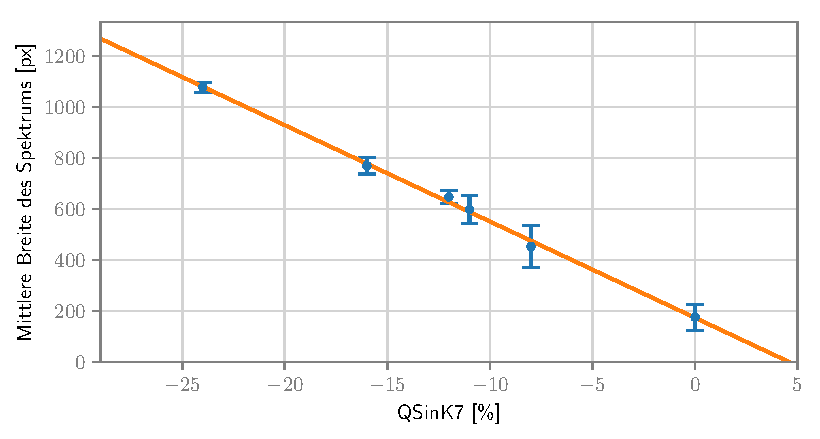
\includegraphics[width=1\linewidth]{../../Jupyter-Notebooks/Kapitel2/Bilder/QSinK7_SM315_width-vs-QSinK7}
	\caption{Mittlere Breite der SR-EEL Spektren in Abhängigkeit von \texttt{QSinK7} für den SpecMag Wert \SI{315}{x}.}
	\label{fig:SR-EELS_Charakterisierung_QSinK7_SM315_QSinK7}
\end{figure}

\begin{figure}
	\centering
	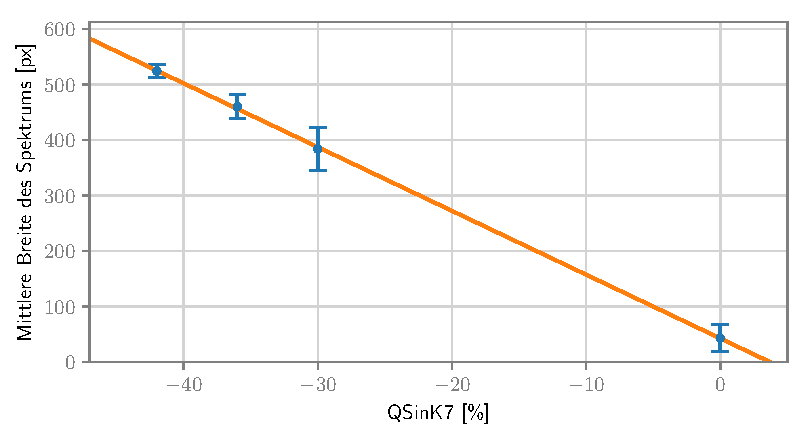
\includegraphics[width=1\textwidth]{../../Jupyter-Notebooks/Kapitel2/Bilder/QSinK7_SM100_width-vs-QSinK7}
	\caption{Mittlere Breite der SR-EEL Spektren in Abhängigkeit von QSinK7 für den SpecMag-Wert \SI{100}{x}.}
	\label{fig:SR-EELS_Charakterisierung_QSinK7_SM100_QSinK7}
\end{figure}

\begin{figure}
	\centering
	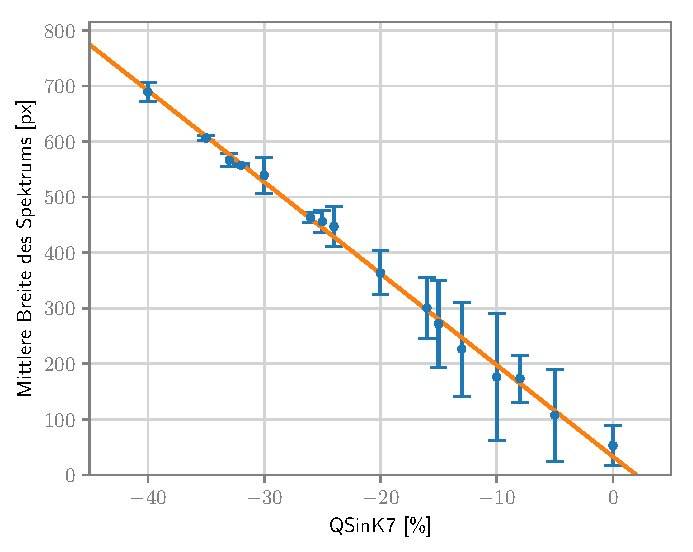
\includegraphics[width=1\linewidth]{../../Jupyter-Notebooks/Kapitel2/Bilder/QSinK7_SM125_width-vs-QSinK7}
	\caption{Mittlere Breite der SR-EEL Spektren in Abhängigkeit von \texttt{QSinK7} für den SpecMag Wert \SI{125}{x}.}
	\label{fig:SR-EELS_Charakterisierung_QSinK7_SM125_QSinK7}
\end{figure}

\begin{figure}
	\centering
	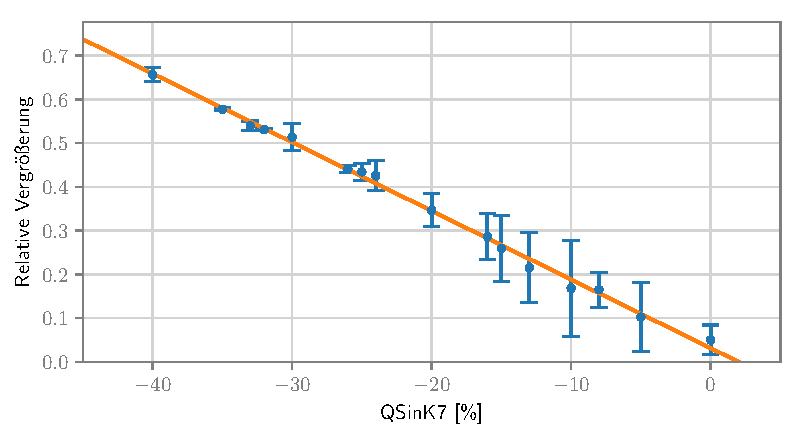
\includegraphics[width=1\linewidth]{../../Jupyter-Notebooks/Kapitel2/Bilder/QSinK7_SM125_width-vs-QSinK7_norm}
	\caption{Relative Vergrößerung der SR-EEL Spektren in Abhängigkeit von \texttt{QSinK7} für den SpecMag Wert \SI{125}{x}. 1 entspricht der Vergrößerung im Abbildungsmodus.}
	\label{fig:SR-EELS_Charakterisierung_QSinK7_SM125_QSinK7_norm}
\end{figure}

\begin{figure}
	\centering
	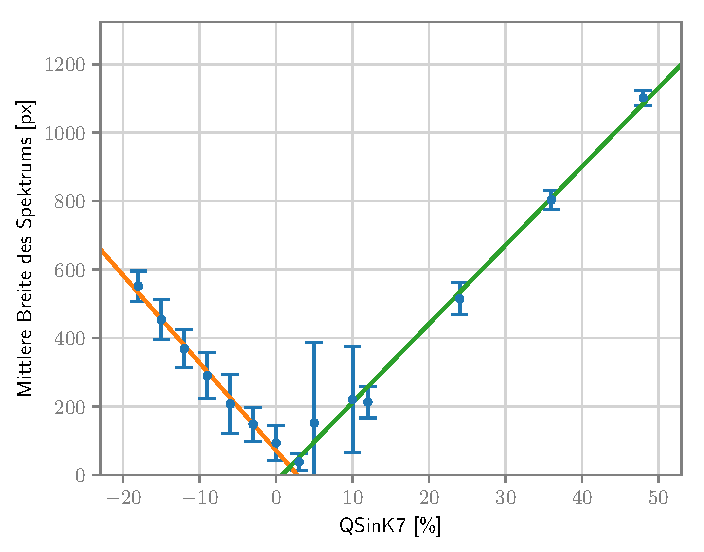
\includegraphics[width=1\textwidth]{../../Jupyter-Notebooks/Kapitel2/Bilder/QSinK7_SM200_width-vs-QSinK7}
	\caption{Mittlere Breite der SR-EEL Spektren in Abhängigkeit von QSinK7 für den SpecMag-Wert \SI{200}{x}.}
	\label{fig:SR-EELS_Charakterisierung_QSinK7_SM200_QSinK7}
\end{figure}

\clearpage

\bibliographystyle{../myamsalpha}
\bibliography{../Literatur}

\end{document}